%&latex
%
\providecommand{\main}{../..}
\documentclass[../../main.tex]{subfiles}

%TO DO: REVIEW AND COMPLETE

\begin{document}
\lesson{5}{18/3/20}

\subsubsection{Calculation of $\Omega(\mathcal{E},N,V)$ for the Ideal Gas (IG)}
Recall that:
\begin{align} \label{eqn:omega-back}
    \Omega(\mathcal{E},N,V) &= V^N \Omega(\mathcal{E},1,N) \equiv V^N \Omega_1(\mathcal{E},N)\\ \nonumber
    \Omega_1(\mathcal{E},N) &= \int_{\mathbb{R}^{3N}} \dd[3N]{\mathbb{P}} \delta\left(\mathcal{E}-\frac{\norm{\mathbb{P}}^2}{2m} \right) = \mathcal{E}^{\frac{3N}{2}-1 } (2m)^{\frac{3N}{2}} \Omega_1(N) \\ \nonumber %Add refs TO DO
    \Omega_1(N) &\equiv \int_{\mathbb{R}^{3N}} \dd[3N]{\mathbb{X}}\, \delta(1-\norm{\mathbb{X}}^2) 
\end{align}
Let us introduce the volume of a $d$-dimensional sphere of radius $\sqrt{\alpha}$:
\begin{align*}
    F_d(\alpha) \equiv \int_{\mathbb{R}^d} \dd[d]{\bm{x}} \theta(\alpha - \norm{\bm{x}}^2)
\end{align*}
Differentiating:
\begin{align*}
    F_d'(\alpha) = \dv{\alpha} F_d(\alpha) = \int_{\mathbb{R}^d} \dd[d]{\bm{x}} \delta(\alpha - \norm{\bm{x}}^2)
\end{align*}
as the \textit{distributional} derivative of a Heaviside function is the Dirac-delta. Note that:
\begin{align}\label{eqn:omega-rel}
    F_{3N}'(1) = \Omega_1(N)
\end{align}

So all that's left is to compute $F_d$. We start from the following identities:
\begin{align*}
    I &\equiv \int_0^\infty \dd{\alpha} e^{-\alpha} F_d'(\alpha) = \int_0^{\infty} \dd{\alpha} \int_{\mathbb{R}^d} \dd[d]{\bm{x}} \delta(\alpha - \norm{\bm{x}}^2) =\\
    &= \int_{\mathbb{R}^d} \dd[d]{\bm{x}} e^{-\norm{\bm{x}}^2} = \pi^{d/2}
\end{align*}
On the other hand, if we instead integrate by parts:
\begin{align}\label{eqn:Fd2}
    I = \int_0^{\infty} \dd{\alpha} e^{-\alpha} F_d'(\alpha) = F_d(\alpha) e^{-\alpha} \Big|_0^{+\infty} + \int_0^{+\infty} F_d(\alpha) e^{-\alpha} \dd{\alpha}
\end{align}
Since $\norm{\bm{x}}^2 \geq 0$, with the equality happening only for $\bm{x} = \bm{0}$, we have that $F_d(\alpha)\Big|_{\alpha = 0} = 0$, and so the boundary term in (\ref{eqn:Fd2}) disappears.

Furthermore:
\begin{align*}
    F_d(\alpha) &= \alpha^{d/2} F_d(1) \Rightarrow F_d(\alpha) e^{-\alpha} \Big|_{0}^{+\infty} = 0 \Rightarrow I= F_d(1) \int_0^{\infty} \alpha^{d/2} e^{-\alpha} \dd{\alpha} = F_d(1) \Gamma\left(\frac{d}{2} +1 \right)
\end{align*}

Comparing the two results for $I$ we get:
\begin{align} \label{eqn:volume-hyper}
    F_d(\alpha) = \alpha^{d/2} F_d(1) = \frac{(\alpha \pi)^{d/2}}{\Gamma\left(\frac{d}{2}+1 \right)}
\end{align}
Substituting back in (\ref{eqn:omega-rel}):
\begin{align*}
    \Omega_1(N) = \frac{3N}{2} \frac{\pi^{3N/2}}{\Gamma\left(\frac{3N}{2}+1 \right)}  = \frac{\pi^{3N/2}}{\Gamma\left(\frac{3N}{2} \right)} 
\end{align*}

Going back through (\ref{eqn:omega-back}) we arrive to:
\begin{align}\label{eqn:final-omega}
    \Omega(\mathcal{E}, V, N) =  V^N \mathcal{E}^{\frac{3N}{2} -1 } \frac{(2 \pi m)^{\frac{3N}{2} }}{\Gamma\left(\frac{3N}{2} \right)} 
\end{align}

\begin{exo}[Verifications]
    Verify:
    \begin{align*}
        \lim_{N \to \infty} N^{-3/2} \frac{\Omega_1(N-1)}{\Omega_1(N)}  = \left(\frac{3}{2 \pi} \right)^{3/2}
    \end{align*}
    using (\ref{eqn:final-omega}) and Stirling's approximation.
\end{exo}

\begin{exo}[Surface area of a hypersphere]
    Use the formula for the volume of a hyper-sphere of dimension $d$ that we obtained in (\ref{eqn:volume-hyper}) to compute the surface area $S_d(r)$ of a $d$-dimensional sphere of radius $r$.
\end{exo}

Before proceeding we want to notice an important property of $\Omega$. In eq (13) $\Omega$ is just a normalization constant for the microcanonical distribution. Since in the averages, such as (14), we have:
\begin{align*}
    \frac{\dd{\Gamma}}{\Omega} = \frac{1}{\Omega} \dd[3N]{\mathbb{Q}} \dd[3N]{\mathbb{P}} 
\end{align*}
we have the freedom to modify slightly the definition of $\Omega$ by re-defining the volume element $\dd{\Gamma}$ of the phase-space by introducing a constant, $h$, with dimension of $q_\alpha \cdot p_\alpha$:
\begin{align*}
    [h] = [q_\alpha \cdot p_{\alpha}] = \si{m}\cdot  \si{\kilo\g \m \per \s} = \si{\s} \cdot \si{\kilo\g} \left(\frac{\si{\m}}{\si{\s}} \right)^2 = [t \cdot \mathcal{E}]
\end{align*}
where $t$ is the time. We will come back later on its physical meaning. At the moment it is just an arbitrary constant whose specific value is not a concern for now. If we redefine:
\begin{align*}
    \dd{\Gamma} = \frac{\dd[3N]{\mathbb{Q}}\dd[3N]{\mathbb{P}}}{h^{3N}} 
\end{align*}
we have that $\dd{\Gamma}$ is a dimensionless volume element. So, for equation (14) to remain valid we must also re-define $\Omega$ as follows:
\begin{align}\label{eqn:omega-redef}
    \Omega(\mathcal{E}, V, N) = \int_{\mathbb{R}^{6N}} \dd{\Gamma} \delta\left(\mathcal{E}- H (\mathbb{Q},\mathbb{P})\right) = \int_{\mathbb{R}^{6N}} \frac{\dd[3N]{\mathbb{Q}} \dd[3N]{\mathbb{P}}}{h^{3N}}  \delta(\mathcal{E}- H(\mathbb{Q},\mathbb{P}))
\end{align}
that is the previously defined $\Omega$ divided by $h^{3N}$. With this redefinition $\Omega$ is also dimensionless, and so we can determine its logarithm for the \textit{particular case} of the IG:
\begin{align} \nonumber
    \Omega(\mathcal{E}, V, N) &= \frac{V^N \mathcal{E}^{\frac{3N}{2} - 1 } (2 \pi m)^{\frac{3N}{2} }}{\Gamma\left(\frac{3N}{2} \right) h^{3N}}\\
\ln \Omega (\mathcal{E}, V, N) &= N\left\{ \frac{3}{2} + \ln\left[\frac{V}{N} \left(\frac{\mathcal{E}}{N} \right)^{3/2} \frac{4 \pi m}{h^3}  \right] + \ln N  \right\} \label{eqn:lnOmega}
\end{align} 
where we have neglected orders of $1/N$ inside the brackets. 

\begin{appr}
    Use that $\Gamma\left(\frac{3N}{2}+1 \right) = \frac{3N}{2} \Gamma\left(\frac{3N}{2} \right)$ and Stirling's approximation
\end{appr}

Were not for the $\ln N$ term, we would have that $\ln \Omega$ is \textbf{extensive}, i.e.:
\begin{align}\label{eqn:omega-extensive}
    \ln \Omega(\lambda \mathcal{E}, \lambda V, \lambda N) = \lambda \ln \Omega(\mathcal{E}, V, N) \quad \forall \lambda > 0
\end{align} 
In other words, if we double the system, setting $\lambda=2$, doubling at the same time the number of particles, the volume and the energy, so that the numeric density $N/V$ and the energy per particle $\mathcal{E}/N$ remain the same as in the original system, then $\ln \Omega \to 2 \ln \Omega$.

\medskip

We will see later that the $\ln N$ term in (\ref{eqn:lnOmega}) has to be removed for very important physical reasons. This will be accomplished by redefining (again) $\Omega$. Thus forget it for now, and, as a result, for the IG case (\ref{eqn:omega-extensive}) holds exactly.
\medskip

It can be shown that the property (\ref{eqn:omega-extensive}) holds for a generic system where $U(\mathbb{Q}) \neq 0$, but the resulting forces (4) are short-range, i.e. the force between pairs of particles decreases \textit{sufficiently fast} when their separations diverge. Thus, even if we have derived (\ref{eqn:omega-extensive}) for the IG where $U(\mathbb{Q}) = 0$, its validity is much more general. The property stated in (\ref{eqn:omega-extensive}) is called \textbf{extensivity}. Indeed if we choose $\lambda = 1/N$ (remember it is arbitrary), from (\ref{eqn:omega-extensive})  we get:
\begin{align}\label{eqn:omega-ext}
    \ln \Omega(\mathcal{E}, V, N) = N \ln \Omega\left(\frac{\mathcal{E}}{N}, \frac{V}{N}, 1  \right) \equiv N s\left(\frac{\mathcal{E}}{N}, \frac{V}{N}  \right)
\end{align}
Which is again valid in general for short-range $U(\mathbb{Q})$.

\medskip

Now we leave the IG case, which was serving as an (important) example, and keep in mind the last result (\ref{eqn:omega-ext}). We will come back to the IG later on.

\section{Temperature}
After the break on the IG, we now come back to the general case of the microcanonical distribution (13) with the definitions (43) and (44). Notice that, in general, i.e. apart from the IG case, $\Omega$ is not easy, if not impossible, to determine!

\medskip

Our goal now is to connect our Statistical Mechanics approach to thermodynamics. Thus we need to identify temperature, $T$, pressure $P$, and chemical potential, $\mu$, with the microscopical states. We start with $T$.

\medskip

From thermodynamics we know that two systems in thermal contact reach \textbf{equilibrium} when their temperatures are the same: 

\begin{figure}[htp]
    \centering
    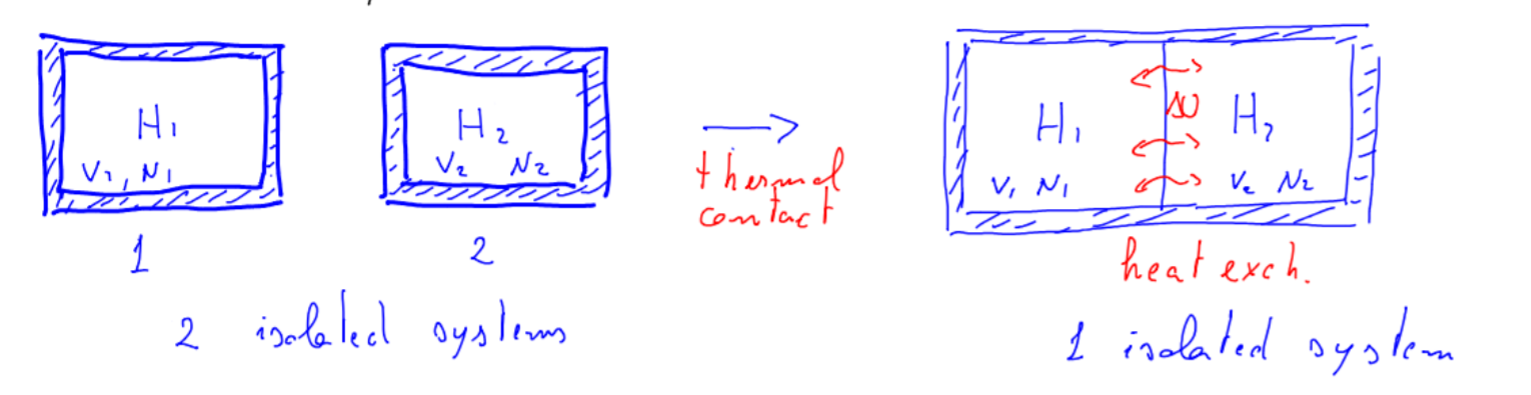
\includegraphics[width=0.9\textwidth]{\main/Images/image003.png}
    \caption{Two isolated systems $1$ and $2$ are \textit{connected} to each other, so that they can exchange energy (but not particles). The larger system will reach equilibrium when the temperatures of \textit{both sides} are the \textbf{same}.\label{fig:thermal-equilibrium}}
\end{figure}

The system on the right corresponds to two interacting systems. The interaction $\Delta U$ between the parts $1$ and $2$ allows the total system to equilibrate, i.e. exchange energy (in the form of \textbf{heat}). Thus the hamiltonian of the entire system is:
\begin{align}\label{eqn:total-H}
    H(\mathbb{Q},\mathbb{P}) = H_1(\mathbb{Q}_1, \mathbb{P}_1) + H_2(\mathbb{Q}_2, \mathbb{P}_2) + \Delta U(\mathbb{Q}_1, \mathbb{Q}_2)
\end{align}
where $\mathbb{Q} = (\mathbb{Q}_1, \mathbb{Q}_2) \in D \subset \mathbb{R}^{3(N_1+N_2)} \ni (\mathbb{P}_1, \mathbb{P}_2) = \mathbb{P}$.

\medskip

In the entire system the conserved quantities are $N_1$, $N_2$, $V_1$, $V_2$ and $H$ (from (\ref{eqn:total-H})). Neither $H_1$ nor $H_2$ are conserved. Thus we can treat the entire (larger) system as a microcanonical ensemble:
\begin{align*}
    \mathcal{P}(\mathbb{Q},\mathbb{P}) = \frac{\delta (\mathcal{E}-H(\mathbb{Q},\mathbb{P}))}{\Omega (\mathcal{E}, V, N)} 
\end{align*}
with $V=V_1 + V_2$ and $N=N_1+N_2$.

\end{document}
